\section{Materiais}
Esta seção descreve os elementos essenciais que viabilizam a condução da pesquisa, contemplando fontes de dados, ferramentas de software e plataformas de hardware utilizadas nas etapas de modelagem, simulação e avaliação do sistema. Esses materiais fornecem o suporte técnico necessário tanto para a construção da base experimental quanto para a execução dos métodos de desenvolvimento e validação apresentados nas subseções seguintes.
\subsection{Base de Dados}

A formação da base de dados é fundamental para o desenvolvimento e validação dos modelos de aprendizado de máquina aplicados à detecção de cavitação. Nesta pesquisa são utilizadas três fontes complementares, abrangendo diferentes contextos experimentais:

\begin{itemize}
	\item \textbf{Falhas em Rolamentos, \textit{Case Western Reserve University, CWRU}:}  
	Conjunto amplamente utilizado na literatura de diagnóstico de falhas, contendo sinais vibracionais sob diferentes cargas e níveis de dano.  
	\textit{Disponível em:} \url{https://engineering.case.edu/bearingdatacenter/download-data-file}
	
	\item \textbf{Cavitação em Bombas, \textit{ UWA System Health Lab}:}  
	Base pertencente à \textit{Prognostics Data Library}, contendo sinais acústicos registrados em condições controladas de cavitação.  
	\textit{Disponível em:} \url{https://systemhealthlab.com/research-tools/prognostics-data-library}
	
	\item \textbf{Bancada Experimental, Projeto MOMEA (Itaipu Binacional / ParqueTec):}
	Conjunto de dados experimentais obtido com o sistema MomeaProbe/MomeaCapture, utilizado para registrar sinais reais de Emissão Acústica (EA) e vibração em motobombas instrumentadas, permitindo a análise detalhada do comportamento dinâmico sob diferentes regimes de carga e escoamento.	
\end{itemize}

A combinação dessas três bases (pública, controlada e experimental) permite avaliar a robustez do modelo em cenários realistas e com diferentes níveis de ruído, abrangendo desde sinais sinteticamente limpos até registros altamente complexos obtidos em operação industrial. Essa diversidade contribui para um processo de validação mais abrangente, capaz de revelar limitações, fortalecer a generalização e orientar ajustes finos da arquitetura rede MLP.


\subsection{Ferramentas e Ambiente de Desenvolvimento}

O desenvolvimento, simulação e avaliação do modelo de Rede Neural Multicamadas
(MLP) em FPGA foram planejados com base no ecossistema de ferramentas da Xilinx,
amplamente utilizado tanto em ambientes acadêmicos quanto industriais. A
plataforma de hardware considerada neste trabalho é a placa Arty A7-35T,
baseada no FPGA Xilinx Artix-7 XC7A35T, que oferece recursos adequados para
prototipagem de sistemas embarcados e aplicações de inferência em tempo real.

\subsubsection*{Xilinx Vivado Design Suite}

O Xilinx Vivado Design Suite constitui o ambiente central do fluxo de projeto.
Essa ferramenta é responsável por gerenciar todas as etapas do desenvolvimento,
desde a definição dos pinos do FPGA até a geração do arquivo final de configuração
(\textit{bitstream}) que será carregado no dispositivo XC7A35T.

No contexto deste trabalho, o Vivado é empregado nas fases de \textit{síntese} e
\textit{implementação}, nas quais a descrição do hardware, seja ela proveniente
de código em nível RTL ou de blocos IP gerados por ferramentas de síntese em alto
nível, é transformada em uma rede física de portas lógicas, interconexões e
registradores dentro do FPGA. Essas etapas permitem avaliar métricas como
utilização de recursos lógicos (LUTs, FFs, BRAMs e DSPs), frequência máxima de
operação e consumo estimado de potência.

O ambiente Vivado também disponibiliza a ferramenta \textit{IP Integrator}, que
possibilita a construção gráfica de sistemas embarcados por meio da interconexão
de blocos funcionais. Nesse cenário, o bloco correspondente à MLP pode ser
integrado a outros componentes do sistema, como controladores de memória,
interfaces de comunicação e módulos de controle, facilitando a composição de uma
arquitetura completa e modular.

Adicionalmente, o Vivado incorpora um simulador lógico próprio, o
\textit{Vivado Simulator}, utilizado para a verificação funcional do projeto.
Essa ferramenta permite validar o comportamento da MLP em nível lógico antes da
implantação no hardware, contribuindo para a identificação e correção de erros
ainda nas etapas iniciais do desenvolvimento.

\subsubsection*{Vitis HLS}

A ferramenta Vitis HLS desempenha papel fundamental na implementação eficiente
da MLP em FPGA. Por meio da Síntese em Alto Nível (\textit{High-Level Synthesis}),
a arquitetura da rede pode ser descrita em linguagens de alto nível, como C ou
C++, evitando a necessidade de codificar manualmente, em HDL, operações
aritméticas complexas como multiplicações de matrizes e acumulações.

O Vitis HLS permite explorar diversas estratégias de otimização por meio do uso
de diretivas (\textit{pragmas}), as quais orientam o compilador a implementar
operações em paralelo (\textit{loop unrolling}) ou de forma encadeada
(\textit{pipelining}). Essas técnicas são particularmente relevantes para
aplicações de diagnóstico de falhas, pois possibilitam reduzir a latência de
inferência e aumentar a taxa de processamento, mantendo controle \mbox{sobre o uso de
recursos do FPGA.}

Após a validação funcional do código em alto nível, o Vitis HLS gera um bloco de
propriedade intelectual (\textit{IP block}), que pode ser importado diretamente
para o ambiente Vivado e integrado ao sistema por meio do \textit{IP Integrator}.
Esse fluxo facilita a prototipagem rápida e a exploração de diferentes
configurações arquiteturais da MLP.

%\subsubsection*{hls4ml}
%
%Como ferramenta acadêmica de apoio, o \textit{hls4ml} é utilizado para facilitar
%a transposição de modelos de aprendizado profundo treinados em ambiente de
%software para arquiteturas em FPGA. Trata-se de uma biblioteca \textit{open
%	source} que traduz automaticamente modelos desenvolvidos em frameworks de alto
%nível, como Keras, TensorFlow ou PyTorch, em código C++ otimizado para o fluxo do
%Vitis HLS.
%
%No contexto deste trabalho, o hls4ml pode ser empregado como uma ferramenta
%auxiliar para acelerar a geração inicial da arquitetura da MLP, permitindo a
%avaliação de diferentes topologias e configurações de quantização. O código
%gerado pode então ser refinado e integrado ao fluxo padrão de síntese e
%implementação no Vivado, mantendo compatibilidade com o FPGA Arty A7-35T.
%
%A utilização conjunta dessas ferramentas estabelece um fluxo de desenvolvimento
%coerente e flexível, no qual a modelagem em alto nível, a síntese em hardware, a
%simulação funcional e a avaliação de desempenho são integradas de forma
%sistemática, permitindo analisar a viabilidade da implementação da MLP em FPGA
%sob as restrições típicas de aplicações de \textit{Edge AI}.


\section{Metodologia}

A metodologia adotada neste trabalho foi estruturada de modo a integrar, de forma coerente, as etapas de preparação dos sinais, modelagem do classificador e avaliação da viabilidade de implementação em hardware reconfigurável. O desenvolvimento do estudo baseia-se em um pipeline de aprendizado supervisionado orientado a dados rotulados, amplamente adotado em aplicações de processamento de sinais e inteligência artificial embarcada, no qual as fases de aquisição, extração de características, treinamento, validação e inferência são tratadas de maneira sistemática e interdependente.

No contexto deste projeto, tal pipeline é adaptado às particularidades dos sinais de Emissão Acústica (EA) e às restrições impostas pela execução em FPGA, incorporando princípios de engenharia de características, modelagem de redes neurais multicamadas (MLP) e co-projeto entre algoritmo e hardware. Cada etapa do fluxo é concebida não apenas como um pré-processamento isolado, mas como um refinamento progressivo da informação, desde os registros experimentais brutos até a representação numérica compacta e quantizada empregada durante a inferência embarcada.

Essa abordagem permite estabelecer uma relação rastreável entre o fenômeno físico monitorado, a representação matemática dos sinais, a modelagem supervisionada por meio de uma MLP e a análise de viabilidade do modelo frente às limitações de recursos e desempenho típicas de um ambiente de Edge AI, no qual aspectos como latência, consumo de recursos lógicos e precisão numérica assumem papel central.

\noindent
No âmbito deste trabalho, o termo \textit{Edge AI} refere-se à execução local de
modelos de inteligência artificial diretamente no dispositivo de borda, neste
caso, uma FPGA, sem dependência de servidores externos. Esse paradigma permite
reduzir latência, tráfego de dados e consumo energético, tornando a inferência
mais adequada para aplicações de monitoramento contínuo em campo.

Nesta abordagem, o fluxo não visa apenas a extração de padrões, mas a construção de um modelo computacionalmente eficiente, capaz de operar sob as restrições de recursos de uma FPGA. O pipeline metodológico foi, portanto, instanciado nas seguintes fases:

\begin{enumerate}
	 \item \textbf{Seleção:} Etapa dedicada à coleta e curadoria dos sinais experimentais de Emissão Acústica. Inclui a definição dos regimes de operação válidos, exclusão de artefatos ruidosos e identificação das janelas temporais representativas \mbox{dos fenômenos cavitantes.}
	
	\item \textbf{Pré-processamento e Transformação:} Envolve o tratamento de sinais (filtragem, segmentação) e a preparação dos tensores de entrada. Nesta fase, são tomadas decisões críticas para o hardware, como a definição da granularidade das janelas e técnicas de normalização compatíveis com a aritmética de \mbox{ponto fixo ou flutuante do FPGA.}
	
	\item \textbf{Modelagem:} Refere-se à construção do núcleo inteligente do sistema. Consiste na implementação, treinamento e otimização da rede MLP supervisionada. Inclui a busca por arquiteturas eficientes, ajuste de hiperparâmetros e estratégias de quantização (se houver) visando o balanço entre acurácia e ocupação \mbox{de área no dispositivo lógico.}
	
	\item \textbf{Interpretação e Validação:} Análise da capacidade de generalização do modelo frente a dados inéditos. Envolve não apenas métricas clássicas (acurácia, matriz de confusão), mas também a validação da viabilidade de implementação e latência de inferência no contexto industrial.
\end{enumerate}

Com base nessas quatro fases, o trabalho foi estruturado em duas frentes metodológicas complementares: \textbf{métodos de desenvolvimento} e \textbf{métodos de avaliação}. Essa separação tem o propósito de esclarecer o papel de cada etapa dentro do fluxo proposto, diferenciando as ações voltadas ao projeto do modelo das atividades destinadas à análise de seu desempenho.

\subsection{Métodos de Desenvolvimento}

Os métodos de desenvolvimento adotados neste trabalho integram, de forma 
sequencial e iterativa, todas as fases necessárias para construir, treinar e 
preparar um modelo rede MLP para futura execução em hardware reconfigurável. 
Essa frente metodológica abrange desde a preparação inicial dos dados até a 
síntese experimental em FPGA, conforme descrito a seguir.

\begin{enumerate}
	\item \textbf{Aquisição e Pré-processamento:}  
	Esta etapa corresponde às fases de Seleção e Transformação do modelo.  
	Inclui a construção da base de dados a partir dos experimentos realizados 
	com o sistema MomeaProbe/MomeaCapture, remoção de trechos inválidos, 
	correção de descontinuidades e normalização das amplitudes para reduzir 
	efeitos de variação entre sensores.  
	Adicionalmente, os sinais foram segmentados em janelas temporais fixas, 
	adequadas ao treinamento da rede MLP e compatíveis com a futura execução em 
	pipeline no ambiente FPGA.
	
	\item \textbf{Modelagem e Treinamento da rede MLP:}  
	Envolve a definição da arquitetura convolucional, incluindo número de 
	filtros, tamanhos de kernel, funções de ativação, camadas densas e 
	estratégias de regularização.  
	Esta etapa corresponde à fase de Modelagem, em que o modelo aprende 
	padrões temporais associados a condições normais e cavitantes.  
	O treinamento supervisionado foi conduzido com métricas padronizadas, 
	como acurácia, F1-score e matriz de confusão.
	
%	\item \textbf{Quantização e Exportação (Brevitas/QONNX):}  
%	Esta fase prepara o modelo para execução eficiente em FPGA.  
%	Utilizou-se \textit{quantization-aware training}, assegurando que a rede 
%	aprenda já sob as restrições do uso de ponto fixo (tipicamente 8 ou 4 bits).  
%	O modelo treinado é então convertido para QONNX, formato compatível com o 
%	compilador FINN, permitindo mapear operadores convolucionais para 
%	arquiteturas \textit{streaming} de hardware.
%	
%	\item \textbf{Síntese Experimental com o FINN:}  
%	Com o modelo quantizado, procede-se à geração do pipeline 
%	\textit{dataflow}, que organiza as camadas em módulos executáveis no FPGA.  
%	São simulados latência, \textit{throughput}, uso de LUTs, BRAMs, URAMs e DSPs, bem 
%	como o fechamento de temporização para diversas configurações de clock.  
%	Esta etapa atua como um ensaio prévio da implementação física, indicando 
%	a viabilidade embarcada da arquitetura proposta.
\end{enumerate}

\subsection{Métodos de Avaliação}

A avaliação da abordagem foi conduzida em dois níveis complementares, que 
dialogam diretamente com as fases de Mineração e Interpretação do modelo DCBD.

\begin{itemize}
	\item \textbf{Avaliação Funcional da rede MLP:}  
	Esta etapa examina o desempenho do modelo no domínio algorítmico.  
	São calculadas métricas como acurácia, precisão, sensibilidade, 
	especificidade, e analisada a matriz de confusão.  
	Tal avaliação permite verificar se a rede é capaz de distinguir padrões 
	associados à cavitação de forma consistente e se reduz a taxa de falsos 
	positivos e falsos negativos.
	
	\item \textbf{Avaliação da Implementação FPGA (simulada):}  
	Utilizando os relatórios do Vivado, são estimados:  
	\begin{itemize}
		\item Uso de recursos lógicos (LUTs, FFs),  
		\item Consumo de memória interna (BRAM, URAM),  
		\item Número de multiplicadores DSP utilizados,  
		\item Frequência máxima possível após síntese,  
		\item Latência total de inferência (em ciclos e segundos),  
		\item \textit{Throughput} por amostra ou por janela.  
	\end{itemize}
	Essa avaliação determina não apenas a viabilidade de implementação, mas 
	também se o sistema pode operar com atraso aceitável (\textit{near real-time}) 
	para integração futura a um monitoramento industrial contínuo.
\end{itemize}

A combinação dessas duas estratégias permite correlacionar o desempenho teórico 
da rede MLP com sua viabilidade prática enquanto componente de um sistema 
embarcado baseado em FPGA.


\subsection{Simulador}

Como não há implementação física no escopo deste projeto, utilizou-se um 
simulador baseado no Vivado. Esse ambiente permite 
replicar, de forma próxima ao hardware real, o comportamento de um acelerador 
convolucional quantizado. O simulador é capaz de:

\begin{itemize}
	\item Reproduzir a arquitetura \textit{dataflow} gerada, incluindo paralelismo interno, movimentação de dados e estruturação do pipeline;
	
	\item Estimar latência por camada e latência total, considerando o uso de 
	ponto fixo e recursos internos do FPGA;
	
	\item Prever o uso de LUTs, \textit{Flip-Flops}, BRAMs, URAMs e DSPs, indicando possíveis 
	gargalos de área ou limitações de \textit{clock};
	
	\item Simular a inferência quantizada, permitindo analisar o impacto da 
	quantização no desempenho do modelo (ex.: perda de acurácia, saturação, 
	erros de truncamento);
	
	\item Validar funcionalmente o modelo quantizado, assegurando que as 
	operações aritméticas implementadas em hardware reproduzem o comportamento 
	esperado do modelo treinado.
\end{itemize}

A Figura~\ref{fig:fluxograma_geral} apresenta uma visão integrada do fluxo 
metodológico, desde o treinamento offline até a simulação do pipeline 
embarcado, consolidando todas as etapas de pré-processamento, quantização, 
compilação e análise de desempenho.


\begin{figure}[H]
	\centering
	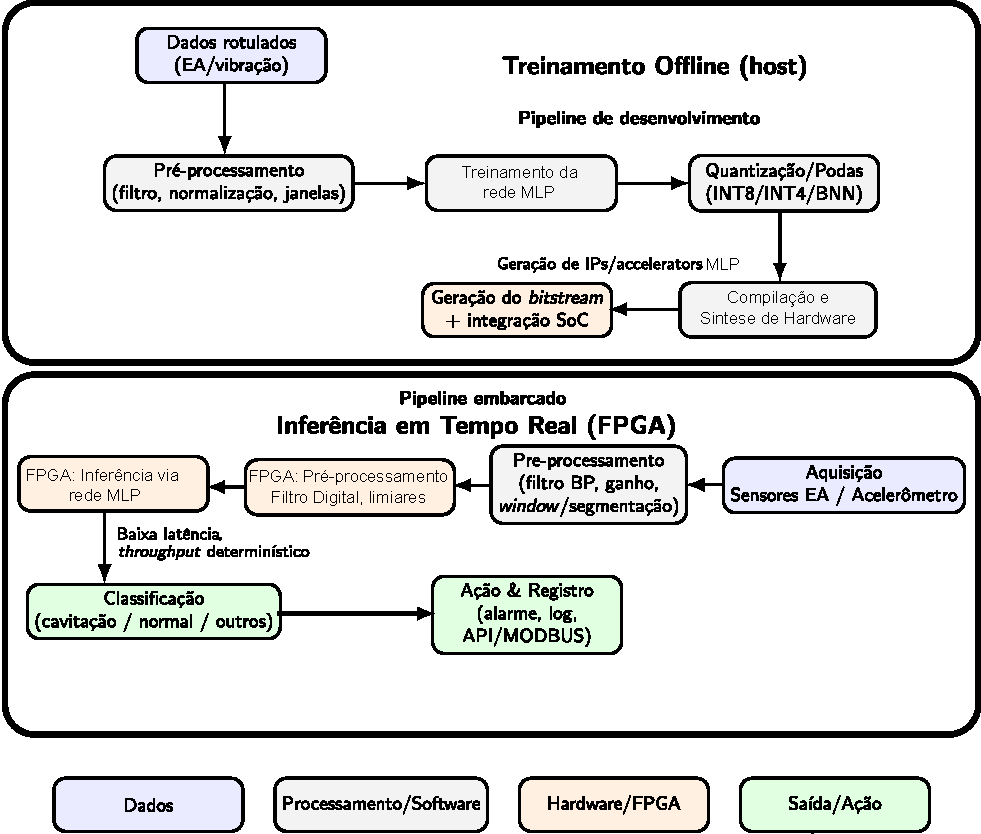
\includegraphics[width=1\linewidth]{figs/Fluxograma_Objetivo_MLP.pdf}
	\caption{Fluxograma geral dos objetivos do projeto, contemplando as etapas de desenvolvimento e inferência da rede MLP em FPGA. Fonte: O autor.}
	\label{fig:fluxograma_geral}
\end{figure}

A Figura \ref{fig:fluxograma_geral} sintetiza o fluxo completo da metodologia adotada neste trabalho, articulando, em um único pipeline, as etapas de treinamento offline e a simulação do pipeline embarcado em FPGA. O diagrama organiza visualmente como os dados brutos de Emissão Acústica são progressivamente transformados até chegar ao núcleo final de inferência, destacando em que ponto cada etapa da metodologia se insere \mbox{e como elas se conectam.}

O fluxo superior representa o Treinamento Offline (host), onde se desenvolve e valida o modelo em ambiente computacional convencional. A partir dos dados rotulados (EA e vibração), aplica-se o pré-processamento, incluindo filtragem, normalização e segmentação em janelas temporais. Os tensores resultantes alimentam o treinamento da rede MLP.

Após o treinamento, o modelo passa pelas etapas de quantização e poda, empregando representações INT8, INT4 ou eventualmente BNN, reduzindo o custo computacional e preparando a rede para execução em hardware reconfigurável. O fluxo culmina na geração do \textit{bitstream} e integração com o ambiente SoC, completando a fase de desenvolvimento.

A metade inferior do diagrama representa o Pipeline embarcado de Inferência em Tempo Real (FPGA). Nele, os sinais provenientes dos sensores de EA e do acelerômetro passam por pré-processamento local, incluindo filtragem passa-banda, ajustes de ganho e segmentação em janelas compatíveis com o acelerador. Esse pré-processamento reduz a variabilidade dos dados e diminui o esforço necessário nas etapas subsequentes.

Os blocos de dados são transferidos para o módulo de inferência por meio de mecanismos de DMA ou FIFO, garantindo fluxo contínuo e latência determinística. A rede MLP compilada é então executada no FPGA, produzindo a classificação entre condições normais, cavitação e outros padrões relevantes. Essa etapa representa a concretização prática da fase de Mineração adaptada ao contexto embarcado.

Os resultados de inferência são entregues ao módulo de Ação e Registro, responsável por alarmes, registro de eventos e comunicação com sistemas externos via API ou MODBUS. Esse bloco completa a fase de Interpretação, traduzindo a saída do modelo para ações operacionais aplicáveis em monitoramento industrial.

Finalmente, a legenda da Figura \ref{fig:fluxograma_geral} organiza os blocos por categoria (dados, processamento, software, hardware, FPGA, saída e ação) reforçando a separação conceitual entre o desenvolvimento offline e a execução embarcada, bem como a continuidade entre ambos.

Dessa forma, o fluxo ilustrado na Figura \ref{fig:fluxograma_geral} não apenas resume a metodologia adotada, mas demonstra a coerência entre a preparação de dados, modelagem, quantização e avaliação em FPGA, evidenciando o alinhamento entre as diferentes fases do projeto e sua orientação a um sistema de inferência eficiente, de baixa latência e adequado para operações quase em tempo real.

Durante o desenvolvimento, serão estabelecidas métricas quantitativas, como latência de inferência, consumo energético, utilização de recursos lógicos e taxa de detecção, que funcionarão como critérios objetivos para avaliar a viabilidade prática da implementação embarcada. Esses indicadores permitirão verificar se o sistema atende às restrições operacionais esperadas e se possui desempenho adequado para aplicação em monitoramento contínuo.

